\documentclass{beamer}
%Information
\title{实习答辩}
\titlegraphic{\hfill
\includegraphics[height=1.5cm]{XJTU.png}}
% \titlegraphic{\hfill\includegraphics[height=1cm]{ORANGE.png}}
\institute{西安交通大学}
\author{王尔卓}
\date{\today}
%Theme
\usetheme[block=fill, sectionpage=none]{metropolis}
\useoutertheme{infolines}
\useinnertheme{metropolis}
\setbeamertemplate{blocks}[rounded][shadow=false]
\setbeamertemplate{items}[ball]
\setbeamertemplate{sections/subsections in toc}[ball]
\setbeamertemplate{headline}{}
\logo{YSA}
\usecolortheme{custom}
%\usetheme{Madrid}
%\usetheme{Heverlee}

%Setting
\usepackage[UTF8,noindent]{ctexcap}
\theoremstyle{definition}
\newtheorem{defn}{Definition}[section]
\newtheorem{coro}[defn]{Corollary}
\newtheorem{theo}[defn]{Theorem}
\newtheorem{exer}[defn]{Exercise}
\newtheorem{rema}[defn]{Remark}
\newtheorem{lem}[defn]{Lemma}
\newtheorem{prop}[defn]{Proposition}
\newtheorem{nota}[defn]{Notation}
\newtheorem{exam}[defn]{Example}
\newtheorem{ques}[defn]{Question}

\newenvironment{prooff}{{\noindent\it\textcolor{cyan!40!black}{Proof}:}\,}{\par}
\newenvironment{proofff}{{\noindent\it\textcolor{cyan!40!black}{Proof of the lemma}:}\,}{\qed \par}
\newcommand{\bbrace}[1]{\left\{ #1 \right\} }
\newcommand{\bb}[1]{\mathbb{#1}}
\newcommand{\p}{^{\prime}}
\renewcommand{\mod}[1]{(\text{mod}\,#1)}
\newcommand{\blue}[1]{\textcolor{blue}{#1}}
\newcommand{\spec}[1]{\text{Spec}({#1})}
\newcommand{\rarr}[1]{\xrightarrow{#1}}
\newcommand{\larr}[1]{\xleftarrow{#1}}
\newcommand{\emptyy}{\underline{\quad}}
\newenvironment{enu}{\begin{enumerate}[(1)]}{\end{enumerate}}
%ctrl+点击文本返回代码  选中代码 ctrl+alt+j 为代码查找文本
\begin{document}
\begin{frame}
    \titlepage
\end{frame}
\begin{frame}{实习企业简介}
    \begin{figure}
        \centering
        
\includegraphics[width=0.3\textwidth]{orange.png}
    \end{figure}
    我的实习公司是北京市青创赢科技教育有限公司, 有一个别称是“工橙院”。
    
    我们公司的主要业务是给北京、杭州等地区的
    小学、初中、高中的国际学校学生提供\blue{计算机留学背景}提升的服务, 准确来说, 是组织学生参加一些计算机相关的
    项目和编程竞赛, 由于申请过程中外方学校还会看中数学相关的竞赛, 因此还会组织一些有认可度的数学竞赛的培训。 
\end{frame}
\begin{frame}{实习企业简介}
国际科技创新大赛项目: 
\begin{enu} 
   \item CS+计算机跨学科文理兼修科研项目
   \item Microsoft lmagine Cup Junior微软创新杯
   \item Kaggle人工智能数据科学挑战赛
   \item 中国青少年科技创新大赛
\end{enu}
国际数学竞赛: 
\begin{enu}
\item CCC 加拿大计算机竞赛
\item USACO 美国计算机奥赛
\item Gauss 加拿大高斯数学竞赛
\item \blue{Euclid 加拿大欧几里得数学竞赛}(每年四月中旬)
\item \blue{AMC8/10/12 美国数学竞赛}()
\end{enu}
\end{frame}
\begin{frame}{AMC比赛简介}
    \begin{table}
        \centering
        \begin{tabular}{c|c|c|c}
            \hline
                     & AMC  8  & AMC 10    & AMC 12    \\
            年级     & $\le 8$ & $\le 10$  & $\le 12$  \\
            开始时间  &每年1月  & 每年11月 & 每年11月     \\
            形式     & 25道题  & 25 道题   & 25 道题   \\
            用时     & 40 分钟 & 75  分钟  & 75  分钟  \\
            总分     & 25      & 150       & 150       \\
            判分方法 & (1,0,0) & (6,1.5,0) & (6,1.5,0) \\
            \hline
        \end{tabular}
    \end{table}
    \begin{itemize}
        \item  $(x,y,z)$为 对一个题$x$分,不填$y$分, 答错$z$分.
    \end{itemize}
\end{frame}
\begin{frame}{AMC 8考察范围}
    \begin{itemize}
        \item 代数: 解方程, 不等式, 数列, 阶乘, 比率.
        \item 组合: 概率, 组合数
        \item 几何: 三角形, 圆形, 矩形, 面积, 角度
        \item 数列: 奇数偶数, 整除, 最大公约数, 唯一因子分解
    \end{itemize}
\end{frame}
\begin{frame}{实习内容简介}
    暑假期间总共带了两个学生, 均为一对一上课, 其中一个学生上了$9$次课, 一个学生上了$6$次, 每节课均为两个小时。
    还有几次试听课, 总时长大约为$35$个小时, 大约从
    教学方式为线上网课, 所选教材为《美国数学竞赛指南。
    \begin{figure}
        \centering
        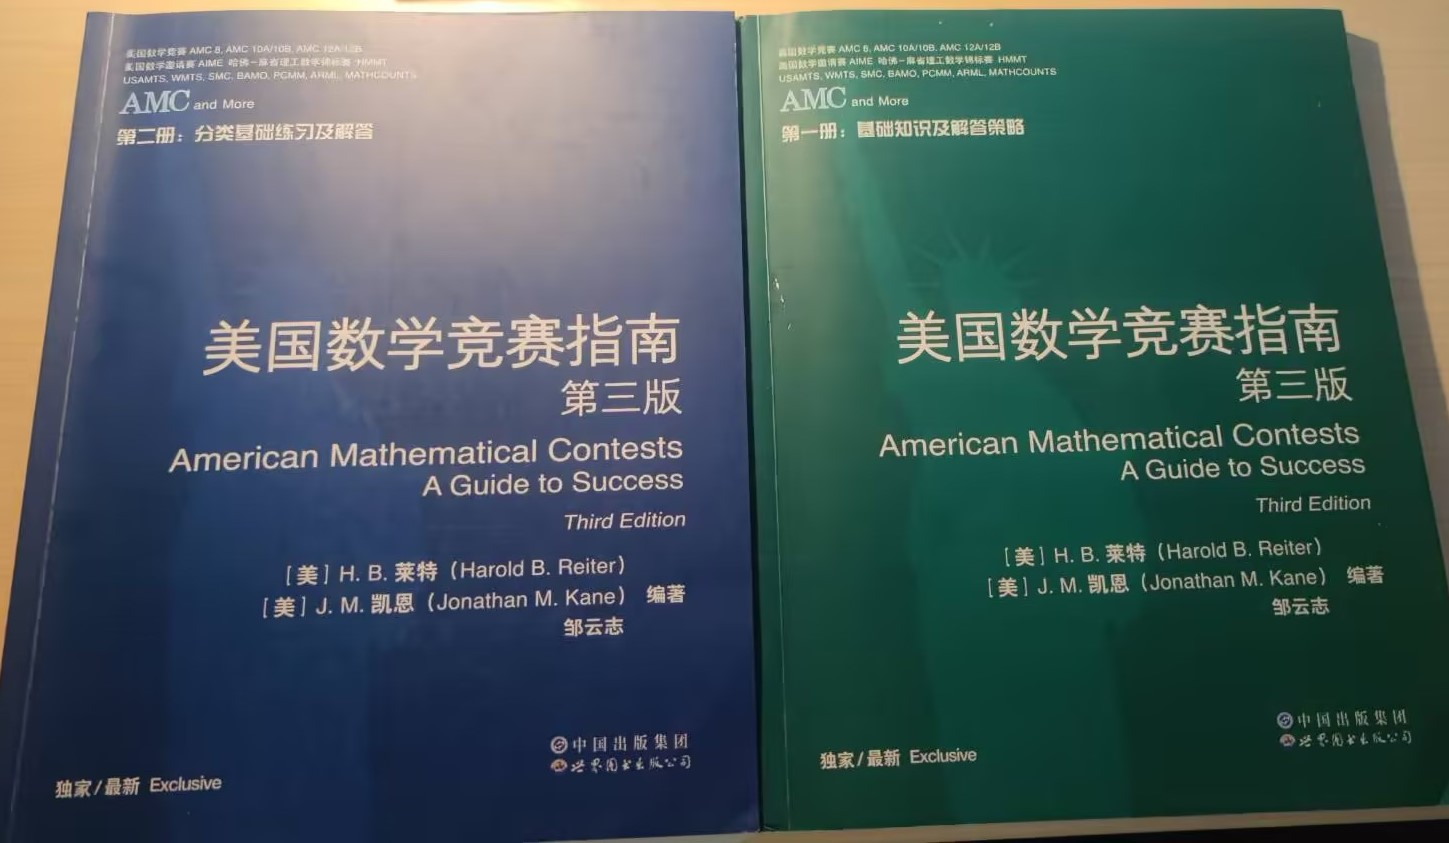
\includegraphics[width=0.5\textwidth]{book.jpg}
    \end{figure}
\end{frame}
\begin{frame}{Introduction}
    In the section, we will study four kinds of arithmetic functions(算术函数/数论函数). 
    They are 
    \begin{itemize}
        \item $\tau(n)=$ the number of positive divisors of $n$.(除数函数)
        \item $\sigma(n)=$ the sum of the positive divisors of $n$.(除数和函数)
        \item $\phi(n)=$ the number of positive integers less than $n$ that are relatively prime to $n$.(欧拉函数)
        \item $\nu_p(n)=$ the exponent of the largest power of $p$.($n$唯一因子分解中$p$的幂次)
    \end{itemize}
\end{frame}
\begin{frame}{$\sigma(n)$}
    If the positive integer $n$ has the prime factorization $n=p_1^{k_1} p_2^{k_2} \cdots p_m^{k_m}$, then the sum of the positive divisors of $n$ is given by
    $$
    \sigma(n)=\frac{p_1^{k_1+1}-1}{p_1-1} \cdot \frac{p_2^{k_2+1}-1}{p_2-1} \cdot \frac{p_3^{k_3+1}-1}{p_3-1} \cdots \frac{p_m^{k_m+1}-1}{p_m-1}
    $$
\end{frame}
\begin{frame}{$\tau(n)$}
    \begin{theo}
        If the positive integer $n$ has the prime factorization $n=p_1^{k_1} p_2^{k_2} \cdots p_m^{k_m}$, then the number of positive divisors of $n$ is given by
        $$
        \tau(n)=\left(k_1+1\right)\left(k_2+1\right) \cdots\left(k_m+1\right) \text {. }
        $$
    \end{theo}
    \begin{exer} 
      How many ordered positive integer pairs $(a,b)$ satisfying $ab=100$?

      有多少个正整数$(a,b)$对满足$ab=100$.

    \end{exer}
\end{frame}
\begin{frame}{Odd $\tau(n)$}
    \begin{prop}
        $\tau(n)$ is odd if and only if $n$ is a perfect quare.

        $\tau(n)$是奇数当且仅当$n$是完全平方数.
    \end{prop}
    \pause 
    \begin{prooff}
        A natural number $n$ has an odd number of divisors exactly when $n$ is a perfect square. Indeed, if $n$ has prime factorization $p_1^{k_1} p_2^{k_2} \cdots p_m^{k_m}$, 
        then $\tau(n)=\left(k_1+1\right)\left(k_2+1\right) \cdots\left(k_m+1\right)$ is odd only if each of its factors is odd, and this happens exactly when each of the exponents $k_1, k_2, \ldots k_m$ are even. That means that $n$ is a perfect square.
    \end{prooff}
\end{frame}
\begin{frame}{$\phi(n)$}
\begin{theo}
If the positive integer $n$ has prime factorization $n=p_1^{k_1} p_2^{k_2} \cdots p_m^{k_m}$, then the number of positive integers less than $n$ that are relatively prime to $n$ is given by
$$
\begin{aligned}
\phi(n) & =n\left(1-\frac{1}{p_1}\right)\left(1-\frac{1}{p_2}\right) \cdots\left(1-\frac{1}{p_m}\right) \\
& =\left(p_1^{k_1}-p_1^{k_1-1}\right)\left(p_2^{k_2}-p_2^{k_2-1}\right) \cdots\left(p_m^{k_m}-p_m^{k_m-1}\right)
\end{aligned}
$$
\end{theo}
\begin{exam}
For example, $\phi(7)=6, \phi(10)=4$, and $\phi(p)=p-1$ if $p$ is prime.
\end{exam}
\end{frame}
\begin{frame}{floor function(高斯函数)}
\begin{defn} 
$\left\lfloor x\right\rfloor=$ 不超过$x$的最大整数.
\end{defn}
\begin{prop}
    $m$ 是一个正整数, $1,2,3\dots,n$中恰有$\left\lfloor \frac{n}{m}\right\rfloor$个数被$m$整除.
\end{prop}
\begin{exam}
    $1,2,3\dots,100$中恰有$\left\lfloor \frac{100}{3}\right\rfloor=33$个数被$3$整除.
\end{exam}
\end{frame}
\begin{frame}{Legendre's formula(勒让德公式)}
    \begin{theo}
        For any prime number $p$ and any positive integer $n$, let $\nu_p(n)$ be the exponent of the largest power of $p$ that divides $n$ (that is, the $p$-adic valuation of $n$ ). Then
        $$
        \nu_p(n!)=\sum_{i=1}^{\infty}\left\lfloor\frac{n}{p^i}\right\rfloor
        $$
        where $\lfloor x\rfloor$ is the floor function.
    \end{theo}
\end{frame}
\begin{frame}{Exercise}
    \begin{ques}[AMC 8, 2017-19]
        For any positive integer $M$, the notation $M!$ denotes the product of the integers 
        1 through M . What is the largest integer $n$ for which $5^n$ is a factor of the sum $98!+99!+100!?$
    
        计算$\nu_5(98!+99!+100!)$.
    \end{ques}
    \pause 
    \begin{prooff} 
        Factoring out $98!+99!+100!$ ,
        we have $98!(1+99+99\times 100)$, which is $98!(10000)$. 
        And $98!$ has $\left\lfloor\frac{98}{5}\right\rfloor+\left\lfloor\frac{98}{25}\right\rfloor=19+3=22$ 
        factors of 5. 
    \end{prooff}
\end{frame}
\begin{frame}{Homework}
    \begin{ques}[AMC 8, 2018-18]
        How many positive factors does 23,232 have?

        23232有多少个正因子?
    \end{ques}
    \begin{ques}[AMC 10, 2005A-15]
        How many positive cubes divide $3!5!7!$? 

        有多少个完全立方数(形如$n=k^3,k\ge 1$) 能整除$3!5!7!$.
    \end{ques}
    \begin{ques}
        What's is the largest power of $2$ that divides the number $K=75!-71!$.

        计算$\nu_2(75!-71!)$.
    \end{ques}
\end{frame}
\begin{frame}{实习的收获}
    经过这十几节课AMC8的教学经历, 我主要有以下几点收获:
    \begin{enu}
      \item 教学时, 要使用通俗易懂的语言讲解。尤其是对抽象能力比较差的学生, 对他们而言讲解一个公式用
      一堆符号和字母来叙述不如使用具体的数字来讲。 
      \item 制作课件时, 如何合理安排习题和讲课的内容, 如何避免内容制作过多或者偏少的问题。要根据不同学生的能力来制作课件, 
      如果内容过难容易让学生产生畏难心理, 望而生畏, 从而打击学生学习积极性。
      \item 与家长沟通时, 要注意沟通方式, 及时消除误解, 不要因为教学上一些细节为向家长解释清楚从而退费。
      比如, 家长可能会对教学方式是不是过于抽象, 以及解法是否简单易懂, 以及内容安排是否合理产生疑问,
      这个时候要及时和家长沟通来解决。
\end{enu}

\end{frame}
\end{document}